\chapter{Introducción}
\label{cap:introduccion}


\section{Contexto}

Las redes Peer-to-Peer (P2P) representan un modelo de comunicación descentralizado en el que todos los nodos participan de forma equitativa, actuando tanto como clientes como servidores.
Este modelo de comunicación, ofrece una alternativa al modelo cliente-servidor tradicional, transformando la forma en que compartimos información.
Una de las áreas donde su impacto es más notable es en el intercambio de archivos, gracias a su capacidad para distribuir grandes cantidades de datos sin depender de servidores centralizados ha supuesto una revolución \cite{schollmeier2001}.

\begin{figure}[h]
    \centering
    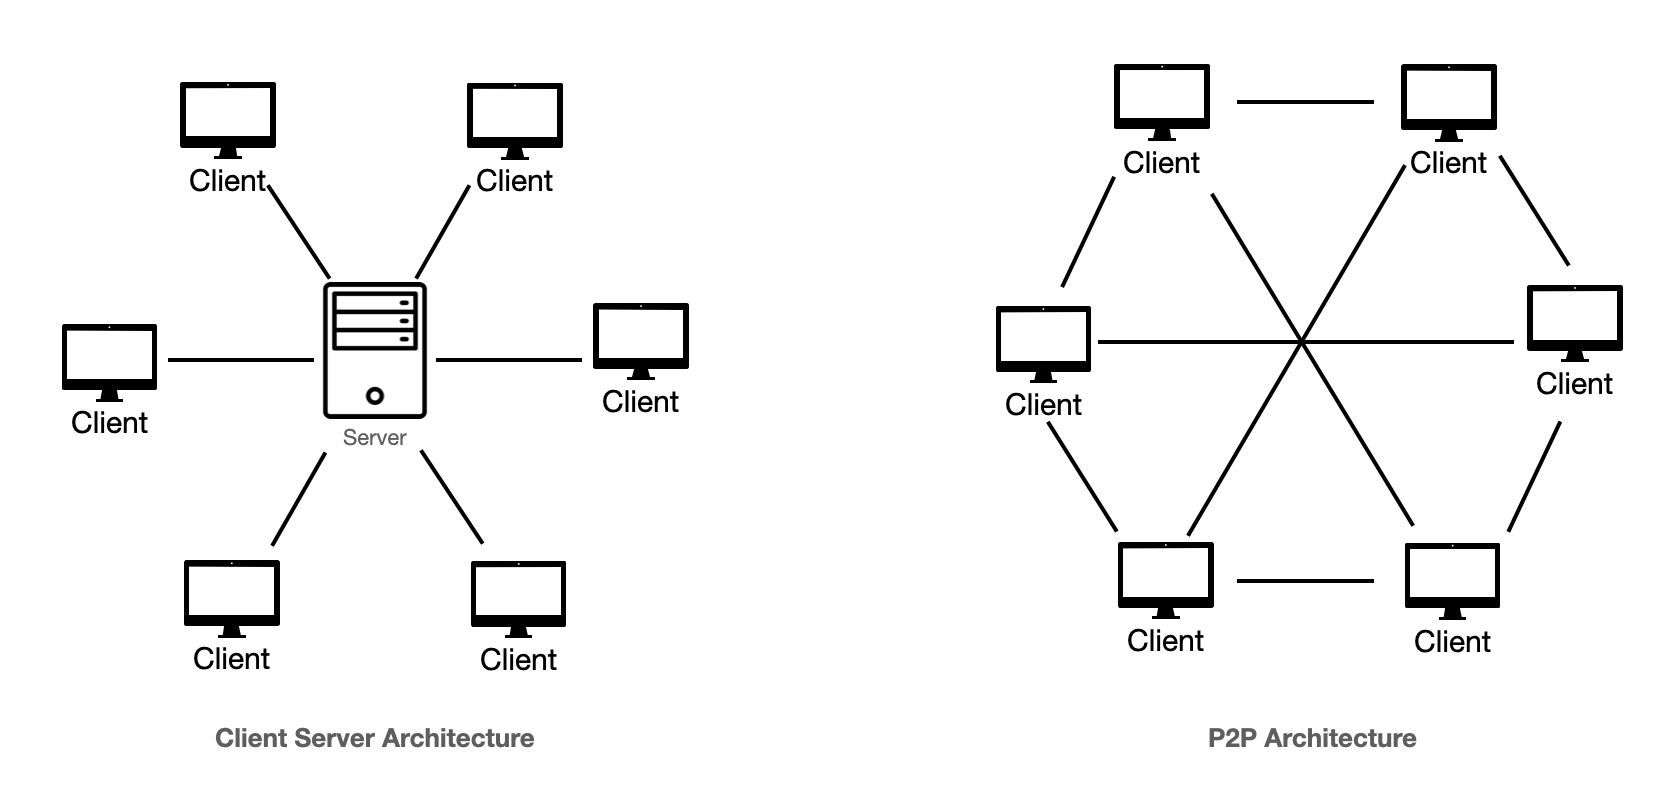
\includegraphics[width = 0.5\textwidth]{Imagenes/Vectorial/client-server-vs-p2p}
    \caption{Comparaci\'on entre arquitectura cliente-servidor y arquitectura P2P}
    \label{fig:clientVsp2p}
\end{figure}


Las redes P2P han tenido un gran impacto en la democratización del acceso a los recursos.
Al eliminar la necesidad de servidores centralizados, estas redes permiten a los usuarios compartir directamente recursos como archivos, ancho de banda o recursos computacionales.
Esto ha impulsado aplicaciones en dominios como el intercambio de contenido multimedia o la computación distribuida.

Sin embargo, este modelo también plantea algunos retos.
Al no tener un punto central de control, se crea la necesidad de desarrollar algoritmos eficientes para la localización de recursos, gestión del tráfico en la red y seguridad en las comunicaciones.

En la actualidad, las redes P2P son fundamentales en aplicaciones que requieren escalabilidad y descentralización.
Como servicios de streaming o distribución de videojuegos hasta sistemas basados en blockchain como Bitcoin,
estas tecnologías suponen un cambio hacia infraestructuras más descentralizadas.


\section{Motivación}

Las redes P2P han cambiado la manera en que compartimos información,
posicionándose como una alternativa eficiente y escalable al modelo cliente-servidor.
A pesar de su relevancia y aplicaciones actuales en campos como el intercambio de archivos, el streaming de vídeo y las plataformas blockchain,
el diseño e implementación de estas redes desde un nivel práctico sigue siendo un reto para muchos desarrolladores.

Este trabajo no busca desarrollar una red masiva con millones de usuarios, más bien se enfoca en la creación de una red P2P funcional desde cero,
centrándose en los conceptos fundamentales y su implementación práctica.

Con ello, se espera facilitar el entendimiento de este modelo descentralizado y motivar el desarrollo de nuevas aplicaciones basadas en redes P2P.


\section{Objetivos}

El objetivo principal de este trabajo es diseñar e implementar una red P2P funcional para el intercambio de archivos de manera distribuida,
integrando tecnologías como UPnP para la gestión automática de puertos y un sistema centralizado para la localización y conexión de nodos.
Este desarrollo se centrará en la creación de un cliente con interfaz gráfica que sirva como base para todas las funcionalidades de la red.

Para alcanzar este objetivo general, se plantean los siguientes objetivos específicos:

\begin{itemize}
    \item \textbf{Desarrollar un cliente con interfaz gráfica:} Diseñar e implementar una aplicación gráfica que permita a los usuarios compartir y descargar archivos de manera sencilla e intuitiva. Este cliente será el núcleo sobre el cual se integrarán las funcionalidades de la red P2P.

    \item \textbf{Desarrollar un sistema de registro y gestión de nodos:} Desarrollar un sistema centralizado que permita identificar y hacer un seguimiento de los peers conectados a la red, permitiendo su interacción y comunicación.

    \item \textbf{Diseñar e implementar la comunicación directa entre nodos:} Crear un protocolo basado en TCP que permita a los peers establecer la conexión para el intercambio de archivos.

    \item \textbf{Integrar soporte para UPnP:} Automatizar la configuración de puertos en los routers mediante el uso de UPnP, permitiendo una configuración sencilla y accesible para los usuarios.

    \item \textbf{Implementar un sistema de intercambio de archivos distribuido:} Diseñar un modelo que permita a los peers compartir y descargar archivos fragmentados desde múltiples nodos, optimizando el uso de los recursos de la red.

    \item \textbf{Documentar el diseño, implementación y evaluación del sistema:} Elaborar una documentación técnica detallada del desarrollo de la red P2P, incluyendo los algoritmos y tecnologías utilizadas.

\end{itemize}


\section{Plan de trabajo}

Durante el desarrollo del proyecto se ha seguido un plan de trabajo detallado con el objetivo de estructurar las tareas y garantizar el cumplimiento de los objetivos.
La planificación ha permitido organizar de manera eficiente las distintas fases del desarrollo, estableciendo prioridades y tiempos.
El plan de trabajo se ha dividido en los siguientes puntos:

\begin{enumerate}

    \item \textbf{Estudio de las tecnologías a utilizar:}
    Se llevó a cabo un análisis detallado de las tecnologías necesarias para el desarrollo del proyecto, incluyendo protocolos de comunicación como TCP,
    sistemas de apertura de puertos con UPnP y arquitecturas P2P para el intercambio de archivos.
    Este estudio incluyó la búsqueda de documentación técnica, recursos en línea y herramientas que facilitaran el desarrollo.

    \item \textbf{Desarrollo del cliente con interfaz gráfica:}
    Se inició el diseño e implementación en java del cliente gráfico como base del proyecto.
    Este cliente incluye funcionalidades esenciales para compartir y descargar archivos, sirviendo como núcleo sobre el cual se desarrollaron las demás características de la red.
    Durante esta fase, se probaron aspectos básicos de la interacción con el sistema de archivos local.

    \item \textbf{Implementación del sistema de registro de nodos:}
    Se diseñó e implementó un sistema centralizado para gestionar los nodos conectados a la red.
    Este sistema permite registrar los peers activos y facilitar su descubrimiento entre ellos.
    Además, se integró con el cliente para garantizar que los usuarios pudieran conectarse a otros peers de manera sencilla.

    \item \textbf{Diseño e implementación de la comunicación entre nodos:}
    Se desarrolló un protocolo basado en TCP para la conexión directa entre peers.
    Esta etapa incluyó las pruebas para garantizar la fiabilidad y estabilidad de las conexiones.

    \item \textbf{Integración del soporte para UPnP:}
    Se implementó soporte para la configuración automática de puertos mediante UPnP, lo que permitió facilitar la conexión entre nodos en redes con configuraciones complejas,
    eliminando la necesidad de ajustes manuales por parte del usuario.

    \item \textbf{Evaluación y pruebas del sistema:}
    Se llevaron a cabo pruebas funcionales para verificar el funcionamiento de cada componente de la red P2P,
    estas pruebas incluyeron casos con múltiples nodos conectados para garantizar la robustez del sistema.

    \item \textbf{Escritura y revisión de la memoria:}
    Durante las fases de implementación y pruebas, se elaboró la memoria del proyecto, documentando las decisiones tomadas y los resultados obtenidos.

    \item \textbf{Cierre del proyecto:}
    Una vez terminadas todas las fases, se realizó una revisión final de la aplicación y de la memoria, realizando las correcciones necesarias para su entrega final.
    Se verificó que todos los objetivos se hubieran cumplido antes del cierre del proyecto.
\end{enumerate}

En definitiva, un plan de trabajo bien estructurado ha permitido avanzar de manera eficiente y cumplir con los objetivos establecidos dentro del tiempo límite.

\section{Organizaci\'on de la memoria}